\documentclass{ut}
\usepackage{fancyhdr}
\usepackage{hyperref}
\usepackage{amsmath}
\usepackage{xepersian}
\usepackage{ifthen}
\usepackage{multirow}

\pagestyle{fancy}
\lhead{\color{NavyBlue}\textbf{(پاسخ نامه تمرین گراف مقدماتی)}}
\rhead{\color{NavyBlue}ساختمان گسسته}

\title{ پاسخ نامه تمرین گراف مقدماتی }
\course{ساختمان گسسته}

\begin{document}
    \thispagestyle{empty}
    \begin{tabular}{r p{0.2\textwidth} c p{0.18\textwidth} l}
        \multirow{5}{*}{\includegraphics[height=2cm]{ut.png}}
        &&\multirow{2}{*}{\textbf{به نام خدا}}&&
        \multirow{5}{*}{\includegraphics[height=2cm]{fanni.png}}\\
        &&&& \\
        &&&& \\
        &&ساختمان گسسته&& \\
        &&\textbf{پاسخ نامه تمرین گراف مقدماتی}&& \\
        \\
        \href{mailto:saratvk1377@gmail.com}{سارا توکلی} &&&& تاریخ : ۱۳۹۸/۱۲/۲۸ \\
        \hline
    \end{tabular}

\begin{enumerate}
    \item
    فرض کنید در گراف $G$ فقط دو رأس فرد وجود داشته‌باشد، ثابت کنید مسیری بین این دو رأس در $G$ وجود دارد. \\
    {\color{Red} جواب :}
    برای اثبات از برهان خلف استفاده می کنیم. فرض خلف : بین این دو رأس مسیری وجود نداشته باشد. در این صورت این دو رأس در دو مؤلفه همبندی جداگانه قرار می گیرند. پس در مؤلفه همبندی فقط یک رأس با درجه فرد داریم و چون مجموع درجات فرد می شود، تناقض است. پس فرض خلف باطل و حکم ثابت شد.
    \item
    ثابت کنید یک گراف ۳-منتظم رأس برشی دارد اگر و تنها اگر یال برشی داشته‌باشد. \\
    {\color{Red} جواب :}
    ابتدا ثابت می کنیم که اگر در این گراف رأس برشی داشته باشیم، یال برشی داریم.\\
    اگر k رأس برشی باشد، چون درجه آن 3 است، دو حالت داریم : \\
    1)	به دو مؤلفه یال داشته باشد. در این صورت به یکی از مؤلفه ها 2 یال و به دیگری یک یال دارد و می‎ توانیم گراف را به صورت شکل 1 رسم کنیم. بدون کاسته شدن از کلیت مسئله، مولفه‌ای که k به آن یک یال دارد را A و مولفه دیگر را B می‌نامیم. چون k برشی است پس از A به B فقط یک مسیر گذرا از k وجود دارد و چون از A به k نیز فقط یک یال وجود دارد، این یال برشی است.\\
    2)	در غیر این صورت اگر به سه مؤلفه یال داشته باشد، به هریک از 3 مؤلفه، یک یال دارد و می‎توانیم گراف را به صورت شکل 2 رسم کنیم. چون k برشی است و به هر مؤلفه فقط یک یال دارد، پس هرکدام از این یال ها نیز برشی هستند. \\
    \\
    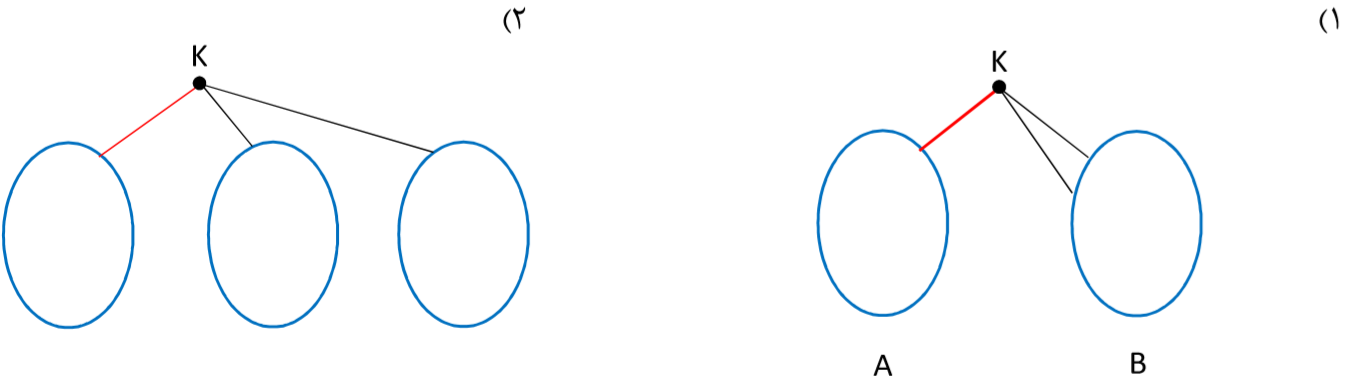
\includegraphics[width=15cm, height=3.5cm]{1.png}\\
    \\
    سپس اثبات می‎کنیم که اگر یال برشی داشته باشیم، رأس برشی داریم.\\
    اگر u یال برشی باشد، می توانیم گراف را مانند شکل زیر رسم کنیم و چون یال u برشی است، بنابراین به جز u یال دیگری از رأس a (یک سر یال u در یک مؤلفه) به مؤلفه دیگر وجود ندارد. بنابراین رأس a نیز برشی است.\\
    \leftline{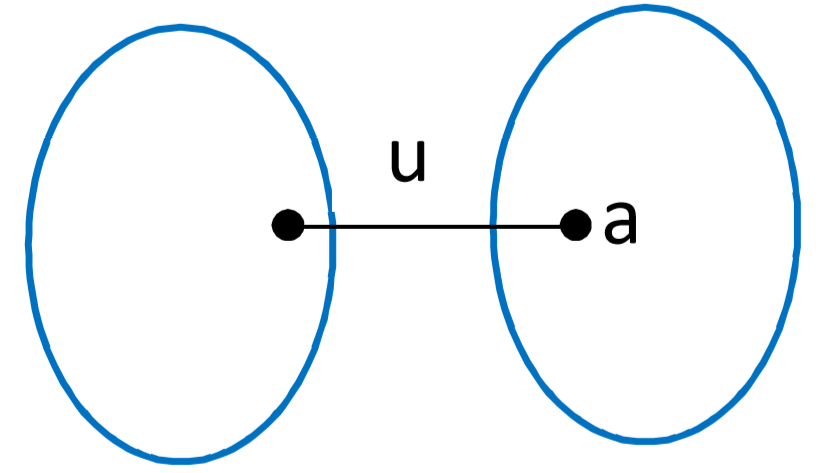
\includegraphics[width=3.3cm, height=2cm]{2.png}}
    \item
    ثابت کنید در گراف سادهٔ $G$ مسیری به طول حداقل $\delta$ وجود دارد.\\
    {\color{Red} جواب :}
    برای اثبات از برهان خلف استفاده می کنیم. فرض خلف : طول بلندترین مسیر $\geq$ 1 - $\delta$\\
    اگر بلندترین مسیر را در این گراف در نظر بگیریم، در این صورت حداکثر $\delta$ تا رأس‌ در این مسیر وجود دارد. چون درجه ی هرکدام از این رئوس حداقل $\delta$ است، بنابراین آخرین رأس این مسیر، حداقل به یک رأس دیگر خارج از این مسیر یال دارد. بنایراین طول مسیر افزایش یافت. که این خلاف فرض خلف است. در نتیجه فرض خلف باطل و حکم ثابت شد.
    \item
    هر یک از رأس‌های گرافی ساده با یکی از دو رنگ آبی و قرمز، رنگ شده‌است. رأس $v$ را ویژه می‌نامیم هرگاه تعداد رأس‌های مجاور $v$ که با $v$ هم‌رنگ هستند از نصف تعداد همسایه‌های $v$ کمتر باشد. در هر گام می‌توانیم یک رأس ویژه را انتخاب و رنگ آن را عوض کنیم. ثابت کنید این عمل پس از مدتی متوقف می‌شود. \\
    {\color{Red} جواب :}
	با ناوردایی مسأله را حل می کنیم. مقدار ناوردا در این مسأله، تعداد یال هایی از گراف است که دو سر آن ها همرنگ می باشد. در هر گام مسأله که یک رأس ویژه را انتخاب و رنگ آن را عوض می کنیم، آن رأس با بیش از نیمی از رأس های مجاور خود، هم رنگ می شود. بنابراین در هر گام، مقدار ناوردا افزایش می یابد و ناوردای افزایشی داریم. چون تعداد یال هایی که دو سر آن ها همرنگ ‎باشد محدود است و نمی تواند از تعداد یال های گراف بیشتر باشد، ناوردا کران دار است و این عمل پس از مدتی خاتمه می یابد و پایان پذیر است.
    \\
    \item
    ثابت گنید تعداد گراف‌های ساده با مجموعهٔ رأس‌های $\{v_{1}, v_{2}, \dots, v_{n}\}$  که درجهٔ هریک از رأس‌های آن‌ها زوج است، برابر است با $2^{{n-1}\choose{2}}$.
    {\color{Red} جواب :}
    اگر A مجموعه همه گراف های ساده با مجموعه رئوس $\{v_{1}, v_{2}, \dots, v_{n-1}\}$ باشد و B مجموعه گراف های ساده با مجموعه رئوس $\{v_{1}, v_{2}, \dots, v_{n}\}$ باشد به گونه ای که درجه تمام رئوس زوج باشد،   
    می دانیم $2^{{n-1}\choose{2}}$ = |A|
    بنابراین می خواهیم تناظر یک به یک بین اعضای مجموعه های A و B برقرار کنیم تا نشان دهیم
    $2^{{n-1}\choose{2}}$ = |B|\\
    اگر G گرافی ساده با مجموعه رئوس $\{v_{1}, v_{2}, \dots, v_{n-1}\}$ باشد، رأس $v_n$ را به آن اضافه می کنیم و آن را به تمام رئوس با درجه فرد وصل می کنیم و و گراف حاصل را G´ می نامیم. 
    بنابراین تمام رئوس با درجه فرد در ،G در G´ درجه زوج دارند. همچنین چون تعداد رئوس با درجه فرد در هر گراف زوج است، پس درجه $v_n$ نیز زوج می باشد. از طرف دیگر اگر برعکس این عمل را روی هر گراف با مجموعه رئوس $\{v_{1}, v_{2}, \dots, v_{n}\}$ که درجه تمام رئوس آن زوج هستند انجام دهیم و رأس $v_n$ را از آن ها حذف کنیم، گرافی ساده با مجموعه رئوس $\{v_{1}, v_{2}, \dots, v_{n-1}\}$ ایجاد می شود. \\
    برای رسیدن از گراف 1 - n رأسی a در A به گراف n رأسی b در ،B به a رأس $v_n$ و یال هایش را اضافه می کنیم و برعکس آن، برای رسیدن از b به ،a رأس $v_n$ و یال هایش را را حذف می کنیم. بنابراین با رفتن از گرافی در A به گرافی در B و برگشتن از B به ،A به همان گراف اول می رسیم. پس تناظر ما یک به یک است.\\
    نکته : برای اثبات تناظر یک به یک، علاوه بر متناظر کردن دو مجموعه به بکدیگر، باید یک به یک بودن این تناظر هم ثابت شود. برای این کار از دو روش می ‎توان استفاده کرد. روش اول مانند اثباتی که قبل تر برای این سوأل آوردیم و روش دیگر این است که نشان دهیم از A به B و از B به A تناظر چند به یک نداریم. به استدلال زیر توجه کنید:\\
    A به B : نشان می دهیم امکان ندارد با اضافه کردن رأس $v_n$ به دو گراف متمایز $a_1$ و $a_2$ از ،A به گراف یکسان b از B برسیم. از برهان خلف  استفاده می کنیم و فرض می کنیم با اضافه کردن رأس $v_n$ به دو گراف متمایز $a_1$ و $a_2$ ، به گراف یکسان b برسیم ( با وجود یکسان بودن گراف های مقصد، آن دو را $b_1$ و $b_2$ می نامیم) . بنابراین رأس $v_n$ در هر دو گراف $b_1$ و $b_2$ با یال های یکسانی وجود دارد و با حذف آن به دو گراف یکسان $a_1$ و $a_2$ می رسیم که با فرض متمایز بودن آن دو تناقض دارد. پس با اضافه کردن رأس $v_n$ به هر دو گراف متمایز از ،A به دو گراف متمایز از B می رسیم.\\
    B به A : با توجه به استدلال بالا و هم چنین چون رئوس برچسب دارند؛ برای هر دو گراف متمایزی، زیر گراف القایی رئوس $v_1$ تا $v_{n-1}$ آن ها از هم متمایز است.\\
    پس چون بین اعضای این دو مجموعه تناظر یک به یک وجود دارد، $2^{{n-1}\choose{2}}$ = |B|\\
    \item
    ثابت کنید $K_{n}$ را می‌توان به ۳ زیرگراف دو به دو ایزومورفیک افراز کرد اگر و تنها اگر $n+1$ بر ۳ بخش‌پذیر نباشد.\\
    {\color{Red} جواب :}
	ابتدا ثابت می کنیم که اگر $K_n$ بتواند به ۳ زیرگراف دو به دو ایزومورفیک افراز شود، n+1 به 3 بخش پذیر نیست.\\
    برهان خلف) فرض خلف: اگر n+1 به 3 بخش پذیر باشد، می‎توان $K_{n}$ را به ۳ زیرگراف دو به دو ایزومورفیک افراز کرد.\\
    می دانیم تعداد یال ها برابر با 
    $\frac{n(n-1)}{2}$ است. چون n+1 به 3 بخش پذیر است، پس n و n-1 به 3 بخش پذیر نیستند. پس نمی توانیم یال ها را به 3 بخش تقسیم کنیم و فرض خلف باطل است.\\
    سپس اثبات می کنیم که اگر n+1 به 3 بخش پذیر نباشد، می توان $K_n$ را به ۳ زیرگراف دو به دو ایزومورفیک افراز کرد.\\
    چون n+1 به 3 بخش پذیر نیست، پس تعداد یال ها به 3 بخش پذیر است. در این صورت 2 حالت داریم:\\
    1) n  به 3 بخش پذیر باشد: برای 2 $\leq$ i $\leq$ 0 ، رأس ها را به سه دسته $v_i$ با اندازه های مساوی تقسیم می‎کنیم. سپس گراف های $G_i$ را به صورت زیر می‎سازیم: (1 + i   و  2 + i  را به پیمانه 3 در نظر بگیرید)\\
    \leftline{یال های درون $v_i$ + یال های بین $v_{i+1}$ و $v_{i+2}$ + کل رأس های گراف = $G_i$}\\
    \\
    2) 1 - n به 3 بخش پذیر باشد: یکی از رئوس گراف ( رأس (u را کنار می‎گذاریم و 1 - n رأس دیگر را، مانند قسمت قبل، به سه بخش  $v_0$ و $v_1$ و $v_2$ با اندازه های مساوی تقسیم می‎کنیم و گراف های $G_0$ و $G_1$ و $G_2$ را تشکیل می دهیم. 
    سپس به ازای 2 $\leq$ i $\leq$ 0،  رأس u را به $G_i$ اضافه کرده و به رأس های $v_i$ وصل می کنیم.
    \item
   ثابت گنید گرافی با $\delta=3$، دارای دور زوج است.\\
   {\color{Red} جواب :}
   یک مسیر ماکسیمال p را در این گراف در نظر بگیرید. اگر v آخرین رأس این مسیر باشد و u رأس قبل  از آن در p باشد، چون مینیمم درجه رئوس 3 است، v باید به غیر از u حداقل به 2 رأس دیگر وصل باشد. چون p ماکسیمال است و v آخرین رأس آن می باشد، پس v نمی تواند به رئوس خارج از p وصل باشد و به جز u به حداقل 2 رأس دیگر در p متصل است. این 2 رأس را x و y می نامیم که به ترتیب دورترین رأس ها از v هستند. 
    \\
    \leftline{{\includegraphics[width=6cm, height=1.8cm]{3.png}}}\\
    \\
    حال در این گراف 3 دور داریم : 1) در مسیر p از x تا v برویم و با یال vx برگردیم. 2) در مسیر p از y تا v برویم و با یال vy برگردیم. 3) در مسیر p از x تا y برویم، سپس با یال yv به v برویم  و با یال vx برگردیم.\\
    پس برای طول دور اول داریم : 2 - ($L_{(2)}$ + $L_{(3)}$) = $L_{(1)}$ .
     بنابراین اگر $L_{(2)}$ و $L_{(3)}$ هردو زوج باشند یا یکی زوج و دیگری فرد باشد، دور به طول زوج داریم. در غیر این صورت اگر هردو فرد باشند، چون مجموعشان زوج است و $L_{(1)}$ با مجموع $L_{(2)}$ و $L_{(3)}$ زوجیت یکسان دارد، پس $L_{(1)}$ زوج است و دور به طول زوج داریم. 
    \item
    ثابت کنید در یک تورنمنت گراف کامل سادهٔ جهت‌دار قویا همبند، به ازای هر $k$ به‌طوری که $3 \leq k \leq n$، دوری جهت‌دار وجود دارد.\\
    {\color{Red} جواب :}
    روی k استقرا می زنیم و داریم: \\
    پایه: 3 = k . رأس v را در نظر بگیرید. اگر رئوسی که به v یال دارند را در مجموعه A و رئوسی که v به آن ها یال دارد را در مجموعه B قرار دهیم، با توجه به این که گراف قویاً همبند است، مجموعه های A و B تهی نیستند و رأس w در B وجود دارد که به رأس u در A یال دارد. بنابر این رئوس w و u و v دور به طول 3 تشکیل می دهند.\\
    \\
    \leftline{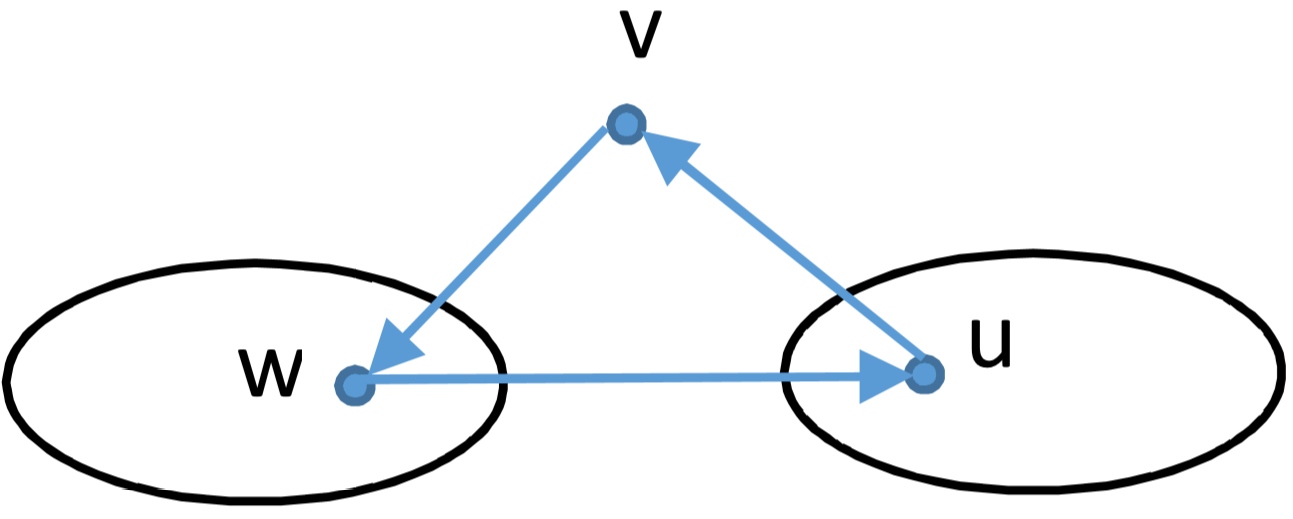
\includegraphics[width=5.4cm, height=2.4cm]{4.png}}\\
    \\
    فرض: دور به طول k داریم.\\\\
    حکم: دور به طول k+1 داریم. \\\\
    دور به طول k را ( با توجه به فرض ) در نظر بگیرید. حال اگر رأس u خارج از این دور وجود داشته باشد که به رئوس داخل دور، هم یال ورودی و هم یال خروجی داشته باشد (حداقل یک یال ورودی و یک یال خروجی)، با توجه به این که گراف تورنومنت قویاً همبند است و u به تمام رئوس داخل دور یال ورودی یا خروجی دارد، رئوس x و y در این دور وجود دارند به طوری که x و y همسایه باشند و از x با یال خروجی به u برویم و با یال ورودی به y برگردیم. پس دور به طول k+1 هم داریم.\\
    در غیر این صورت، اگر رئوسی داشته باشیم که همه به رئوس داخل دور وارد می شوند (مجموعه (A و رئوسی داشته باشیم که همه از آن ها خارج می شوند (مجموعه ،(B چون گراف قویاً همبند است، پس حتماً از B به  A مسیر داریم. پس دور به طول k+1 داریم.\\
    \\
    \leftline{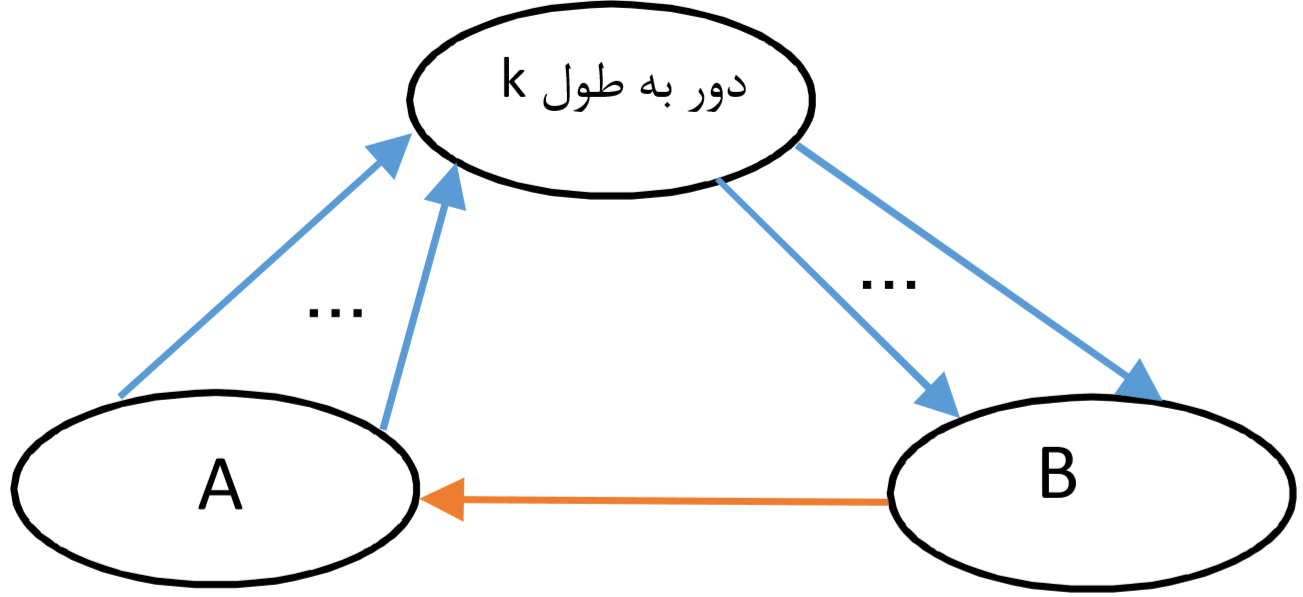
\includegraphics[width=6cm, height=3.2cm]{5.png}}\\
\end{enumerate}

\end{document}
